\section{Einleitung und Motivation}

In diesem Versuch wird mit Hilfe der Faraday-Rotation die effektive Masse des Halbleiters Galliumarsenid bestimmt. Die Faraday-Rotation beschreibt die Drehung der Polarisationsebene einer elektromagnetischen Welle in einem Material unter dem Einfluss eines Magnetfeldes, welches parallel zur Ausbreitungsrichtung der Welle ist. Desweiteren lassen sich mit Hilfe der Faraday-Rotation Informationen über die Bandstruktur der verwendeten Proben gewinnen. 

\section{Theorie}

\subsection{Effektive Masse}
Bei der Beschreibung von komplizierten Bandstrukturen eines Halbleiters lassen sich die physikalischen Effekte mit einer einfachen Approximation beschreiben. In der unteren Abbildung \ref{fig:bandstruktur} wird die vereinfachte Form des Leitungsbandes und des Valenzbandes dargestellt.
\begin{figure}[h!]
	\centering
	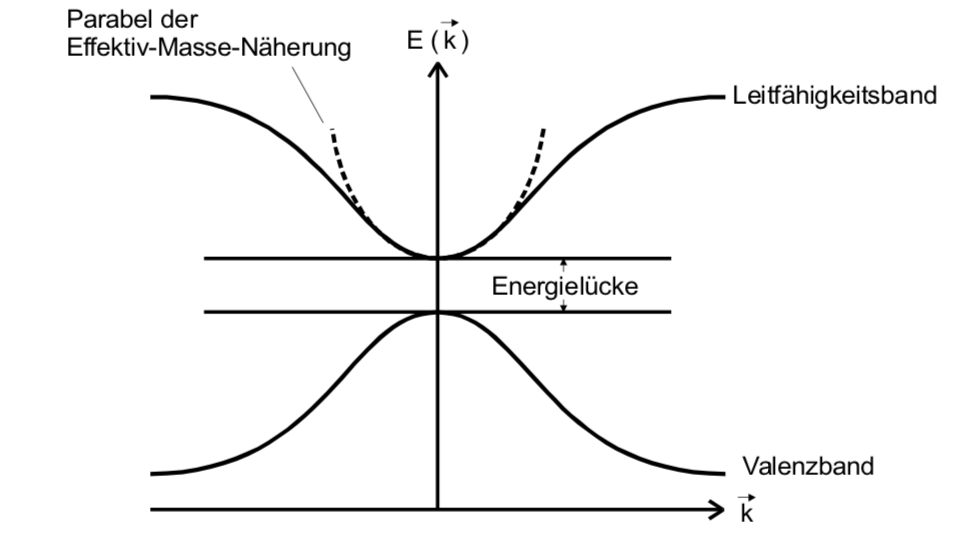
\includegraphics[width=0.7\linewidth]{../../Polina/bandstruktur}
	\caption{Bandstruktur eines Festkörpers, \cite{anleitungV46}.}
	\label{fig:bandstruktur}
\end{figure}
Für die weitere Berechnung wird der Verlauf des Leitungsbandes näher untersucht. Für einen Wellenzahlvektor von $\vec{k}$ mit einem Minimum bei $k=0$ kann die Elektronenenergie $\epsilon$ in eine Taylorreihe entwickelt werden.
\begin{align}
\epsilon(\vec{k})=\epsilon+ \dfrac{\hbar^2k^2}{2m^{\ast}}
\end{align}
Bei hoher Symmetrie des Kristallgitters ergeben sich kugelförmige Energieflächen und $m^{\ast}$ stellt dabei die effektive Masse dar und beträgt
\begin{align}
m^{\ast}=\dfrac{h^2}{\left(\dfrac{\delta^2\epsilon}{\delta k_i^2}\right)_{k=0}}
\end{align}
Diese ist deshalb vom Vorteil, weil Elektronen in einem Band wie freie Teilchen betrachtet werden können und es gilt die Quantenmechanik freier Teilchen. Beim Anlegen eines nicht zu großen äußeren elektrischen oder magnetischen Feldes kann das zweite Newtonsche Grundgesetz angewandt werden und für die weitere Berechnung des Faraday-Effektes die klassische Mechanik genutzt werden. 
\subsection{Zirkulare Doppelbrechung}
Bei der zirkularen Doppelbrechung tritt ein linear polarisierter Lichtstrahl in ein Material ein und ändert nach Austritt die Polarisationsebene. Zur Berechnung des Drehwinkels $\theta$ wird angenommen, dass die Lichtwelle nach Durchtritt durch das Material in eine rechts- und linkszirkuläre Welle zerlegt wird. 
\begin{align}
\label{eq:gl3}
E(z)=\dfrac{1}{2}(E_\text{R}(z)+E_\text{L}(z))
\end{align}
Dabei sind die Phasengeschwindigkeiten von links und rechtszirkulärem Anteil des Lichtes im Material unterschiedlich. Durch Umformen und Zerlegen der Gleichung \ref{eq:gl3} kann ein Ausdruck für den Drehwinkel $\theta$ ermittelt werden. 
\begin{align}
\label{eq:gl4}
\theta= \dfrac{L\omega}{2c} \left(\dfrac{1}{v_{\text{Ph}_R}}-\dfrac{1}{v_{\text{Ph}_L}}\right)
\end{align}
Mit Hilfe der Brechungsindices $n_\text{R}$ und $n_\text{L}$ wird die Gleichung \ref{eq:gl4} zu
\begin{align}
\theta= \dfrac{L\omega}{2} (n_\text{R}-n_\text{L})
\end{align}
L ist hierbei die Länge des Materials und $\omega$ die Kreisfrequenz der einfallenden Welle. Die Doppelbrechung geschieht aufgrund des elektrischen Dipolmomentes, das durch die Atome auf den Gitterplätzen und durch die Wechselwirkung der Bandelektronen mit den Atomrümpfen erzeugt wird. Die Gesamtheit der Dipole pro Volumeneinheit, die als mikroskopische Polarisation bezeichnet wird, beträgt
\begin{align}
\vec{P}=\epsilon_0 \chi \vec{E}
\end{align}
$\chi$ ist die dielektrische Suszeptibilität. Bei isotroper Materie stellt dieser eine skalare Größe dar und bei anisotropen Kristallen einen Tensor dritter Stufe. Nach weiteren Umrechnungen erhält man für den Drehwinkel den Ausdruck 
\begin{align}
\theta= \dfrac{L\omega}{2cn}\chi_{xy}
\end{align}
\subsection{Berechnung des Rotationswinkels beim Faraday Effekt}

Der Faraday Effekt und somit auch die Drehung der Polarisationsebene wird durch das Anlegen eines äußeren Magnetfeldes erzeugt. Dabei kommt es zu einer Wechselwirkung des Magnetfeldes mit den Elektronen der Materie. Für ein gebundenes Elektron gilt die folgende Bewegungsgleichung 
\begin{align}
m\dfrac{d^2\vec{r}}{dt^2}+K\vec{r}=-e_0\vec{E}(r)-e_0\dfrac{d\vec{r}}{dt}\times\vec{B}
\end{align}
Dabei ist $m$ die Masse und $e_0$ die Ladung des Elektrons. Zudem steht $\vec{r}$ für die Auslenkung des Elektrons aus der Gleichgewichtslage, $K$ ist eine Konstante, die seine Bindung an die Umgebung beschreibt und $\vec{E}$ ist die Feldstärke der einfallenden Lichtwelle. Unter der Annahme, dass Dämpfungseffekte und der Einfluss des Magnetfeldes der elektromagnetischen Lichtwelle vernachlässigt werden darf, da sie nur einen geringen Einfluss auf den Faraday-Effekt haben, ergibt sich für den Winkel der Polarisationsebene mit der Proportionalität 
\begin{align}
\vec{P}=-Ne_0\vec{r}
\end{align}
und der Tensorkomponente 
\begin{align}
\chi_{xy}=\dfrac{Ne_0^3\omega B}{\epsilon_0\left(\left(-m\omega^2+K\right)^2-\left(e_0\omega B\right)^2\right)}
\end{align}
der Winkel
\begin{align}
\label{eq:gl11}
\theta=\dfrac{e_0^3}{2\epsilon_0 c}\dfrac{1}{m^2}\dfrac{\omega^2}{\left(-\omega^2+\dfrac{K}{m}\right)^2 -\left(\dfrac{e_0}{m}B\omega\right)^2}  \dfrac{NBL}{n}
\end{align}
mit der Flussdichte $B$, der Probenlänge $L$ und der Zahl der Ladungsträger $N$ pro Volumeneinheit. $\sqrt{\dfrac{K}{m}}$ kann hier als Resonanzfrequenz $\omega_0$ und $\dfrac{Be_0}{m}$ als Zyklotron-Frequenz $\omega_C$ betrachtet werden. Mittels der Annahme, dass die Messfrequenz viel kleiner als $\omega_0$ und dass die Resonanzfrequenz größer als die Zyklotron-Frequenz ist, lässt sich die Gleichung \ref{eq:gl11} schreiben als:
\begin{align}
\theta(\lambda)=\dfrac{2\pi^2 e_0^3 c}{\epsilon_0}\dfrac{1}{m^2}\dfrac{1}{\lambda^2 \omega_0^4}\dfrac{NBL}{n}
\end{align}
Für freie Ladungsträger ergibt sich mittels der Annahme, dass $\omega_0$ gegen Null geht:
\begin{align}
\theta_{frei}=\dfrac{e_0^3\lambda^2}{8 \pi^2 \epsilon_0 c^3 m^2 }\dfrac{NBL}{n}
\end{align}
wird $m$ durch $m^{\ast}$ ersetzt, so erhält man den Zusammenhang zwischen Drehwinkel $\theta$ und der effektiven Masse $m^{\ast}$ der Elektronen im Kristall. 